\documentclass[aps,prl,twocolumn]{revtex4}

\usepackage{amsmath}
\usepackage{amsfonts}
\usepackage[caption=false]{subfig}
\usepackage{graphicx}

\renewcommand{\vec}[1]{\mathbf{#1}}

\newcommand{\mat}[1]{\mathrm{#1}}
\newcommand{\by}{\times}
\newcommand{\of}[1]{\!\left(#1\right)}
\newcommand{\pdf}{{\it pdf}}
\newcommand{\abs}[1]{\left|#1\right|}
\newcommand{\prob}[1]{\mathcal{#1}}
\newcommand{\bosonsampling}{\textsc BosonSampling}
\newcommand{\ket}[1]{\left|#1\right\rangle}

\setlength{\parindent}{0pt}
\setlength{\parskip}{4mm}

\begin{document}

\title{Direct dialling of Haar unitary matrices}

\author{Nicholas J. Russell et al.}
\affiliation{Centre for Quantum Photonics, H. H. Wills Physics Laboratory,
Tyndall Avenue, Bristol, BS8 1TL}

\begin{abstract}
Random unitary matrices are central to the recently defined \bosonsampling{}
problem, which presents a post-classical model of computation implemented by
photons in linear optical circuits. We present a physically-motivated and
compact representation of the probability density function for Haar random
unitary matrices, where each parameter corresponds directly to a physical
component in a linear optical realisation of the unitary. We show how to use
this representation to efficiently generate linear optical circuits
implementing random unitaries and go on to apply the derived methods to qubit
unitaries.
\end{abstract}

\maketitle

\section{revised}
The development of the \bosonsampling{} problem \cite{aa-conf-11-333} has
motivated fresh interest in studying \emph{random} unitaries that describe the
optical circuits acting on multiphoton states. Rapid developments in the field
of integrated optics with reconfigurable components facilitates the construction
of large-scale optical circuits capable of actively realising any unitary
operator. Combined with on-chip sources \cite{si-nphoton-8-104}
and detectors \cite{re-srep-3, pe-ncomm-3-1325}, the scale of experimental
implementations of \bosonsampling{} \cite{cr-nat-7-545, br-sci-339-794,
sp-sci-339-798, ti-nphoton-7-540} is likely to increase.
% ^^
% I'd like to add to this my sentence about not being interested in the exact
% form of the unitary; rather just the distribution

\begin{figure}[t]
  \centering
  \subfloat[]{
    \includegraphics{figures/recursive}
    \label{fig:recursive}
  } \\
  \subfloat[]{
    \includegraphics{figures/cascade}
    \label{fig:cascade}
  }
  \caption{Recursive decomposition of a unitary. \ref{fig:recursive} shows an
    \(m \by m\) unitary as a product of \(m\) unitary transformations
    \(\mat{R}_{i}\), each acting on a successively larger subspace.
    \ref{fig:cascade} expands one of the \(\mat{R}_{i}\) unitaries in terms of
    a cascade of beamsplitters and phase shifts. The connection between the
    \emph{Cartesian} basis, \(\vec{x}\) and the \emph{physical} basis,
    \(\vec{r}\) is illustrated by the labels on \ref{fig:cascade}.}
  \label{fig:reck}
\end{figure}

In linear optics, any unitary operator can be implemented as an array of
beamsplitters and phase shifters as shown in figure~\ref{fig:reck}. A similar
mathematical decomposition has been known for some time in the work of Hurwitz
\cite{hurwitz}, with the link to experimental components made more recently by
Reck et al. \cite{re-prl-73-58}. Here we present a simple procedure for choosing
a Haar random unitary on an optical circuit by choosing values of the physical
parameters independently from simple distributions. This procedure is useful in
applications such as \bosonsampling{} where we do not need to know the exact
unitary description of the circuit being implemented, but need a guarantee that
it is drawn from the correct distribution. While similar parameterisations exist
in the mathematical literature \cite{sp-jmp-53-013501, zy-jpa-27-4235}, the
relevance to linear optics is not widely appreciated. Further, we extend the
result to systems of qubits, by making the connection between a linear-optical
circuit on \(m=2^{n}\) modes and a circuit operating on \(n\) qubits.

We begin by briefly introducing a general unitary parameterisation on an
\(m\)-dimensional space and continue to describe the method for drawing Haar
unitaries in this picture, including a simplo proof of validity. We go on to
explicitly describe a mapping between linear optical circuits and qubit
circuits, and apply the same results to this system.

Drawing a Haar random unitary is analogous to choosing a random number from a
uniform distribution in that it should be unbiased. The probability of drawing
a particular unitary matrix from some region in the space of unitaries should
be in direct proportion to the volume of the region, as defined by the Haar
measure, which is the unique translation-invariant measure on the space of
unitaries \cite{re-phd}. As argued in \cite{re-phd}, if \(m\) vectors \(\left\{
v_{i} \right\} = \left\{ v_{1}, v_{2}, \cdots, v_{m} \right\}\) are successively
drawn from the unbiased distribution of unit vectors in the
\(\left(m-i\right)\)-dimensional subspace orthogonal to all previous vectors,
they form the columns of a Haar random unitary. The problem of choosing Haar
random unitaries thus reduces to the problem of drawing such a set of orthogonal
vectors.

We approach this problem by considering a general linear optical circuit, which
suggests a recursive strategy for achieving the appropriate set of vectors.
Figure~\ref{fig:recursive} shows a recursive strategy for a physical
implementation
of any unitary matrix on \(m\) modes. Each block labelled \(\mat{R}_{n}\) takes
as input the basis state \( \ket{m-n}\) and performs a unitary operation to
produce the \(n\)-dimensional vector \(\ket{v_n}\). Orthogonality is preserved
as this vector is transformed by all subsequent \(\mat{R}_{i}\). Further, if the
vector \(\ket{v_{n}}\) is chosen from the unbiased distribution of unit vectors
in \(n\) dimensions, the property of left invariance ensures that it does not
become biased by the operation of the subsequent \(\mat{R}_{i}\).

The next consideration is therefore how to choose appropriate vectors, i.e.\
unbiased unit vectors, in \(n\) dimensions. Figure~\ref{fig:cascade} expands one
of the \(\mat{R}_{i}\) in terms of linear optical components, and we proceed
from here. Consider the complex Gaussian vector in \(n\) dimensions:
\begin{equation}
  \vec{v}_n = \begin{pmatrix}
    z_0 \\
    z_1 \\
    \vdots \\
    z_{n-1}
  \end{pmatrix}
\end{equation}
where the \(z_i\) are i.i.d. Gaussian complex numbers, \( z \sim \exp \left(
-\abs{z}^2 \right) \). Because of their independence, the probability
density function (\pdf{}) for \(\vec{v}_n\) is the product of the \pdf{}s for
the elements and depends only on the magnitude of the vector. Let \(x_i
= \abs{z_i}^2 \), then:
\begin{equation}
  \label{eq:vec}
  \prob{P}_{\vec{v}_n} = e^{ -\left(x_0 + x_1 + \dots + x_{n-1} \right)} = e^{
  -\abs{\vec{v}_n}^2}
\end{equation}
Now consider the change of variables from this basis~\(\vec{x}\), which we call
the Cartesian basis, to a new basis,~\(\vec{r}\):
\begin{align}
  x_i &= r_0 \left[ \prod_{k=1}^{i} \left( 1-r_k \right) \right] r_{i+1} &
    \left( 0 \leq i < n-1 \right) \\
  x_{n-1} &= r_0 \left[ \prod_{k=1}^{n-1} \left( 1-r_k \right) \right] \\
  r_0 &= \sum_{k=0}^{n-1} x_k \\
  r_i &= \frac{x_{i-1}}{\sum_{k=i}^{n-1} x_k} & \left( 0 < i \leq n-1 \right)
\end{align}
We refer to \(\vec{r}\) as the physical basis because the variables
correspond directly to components in a physical realisation of the vector in
linear optics. In particular, \(r_0\) is the power of the input and the other
\(r_i\) are reflectivities of beamsplitters. The relationship between
\(\vec{x}\), \(\vec{r}\) and the physical system is shown in
figure~\ref{fig:reck}. The phases \(\phi_{ij}\) and \(\alpha_i\) do
not appear in either basis.

In order for this parameterisation to be useful, we must show that the \pdf{}
for the vector \(\vec{v}_n\) is separable in the physical basis so that the
experimental parameters can be chosen independently. We also need to derive the
form of the marginal distributions for the \(r_i\). These will be the
distributions from which experimental parameters must be chosen to obtain a Haar
unitary. The change of variables is performed using the Jacobian, as follows:
\begin{equation}
  \prob{P}_{\vec{v}_n} \of{\vec{r}} = \prob{P}_{\vec{v}_n} \of{\vec{x}}
  \abs{\det \mat{J} \of{\vec{x}, \vec{r}}}
\end{equation}
where
\begin{equation}
  \mat{J}_{ij} \of{\vec{x}, \vec{r}} = \frac{\partial x_{i}}{\partial r_j}
\end{equation}
Equation~\ref{eq:vec} is expressed in the \(\vec{r}\) basis simply as \(\exp
\of{-r_0}\), so is trivially seperable. We now just have to show that the
Jacobian determinant is also seperable.

There are 6 different expressions for elements \(\mat{J}_{ij}\) of the
Jacobian. On the bottom row of the matrix (i.e. \(i=n-1\)) we have:
\begin{align*}
  &\left[ \prod_{k=1}^{n-1} \left( 1-r_k \right) \right]& j &= 0 & \\
  -r_0 &\left[ \prod_{k=1}^{j-1} \left( 1-r_k \right) \right] \left[
  \prod_{k=j+1}^{n-1} \left( 1-r_k \right) \right]& j &> 0
  \intertext{And on all other rows}
  &\left[ \prod_{k=1}^{i} \left( 1-r_k \right) \right] r_{i+1}& j &= 0 \\
  -r_0 &\left[ \prod_{k=1}^{j-1} \left( 1-r_k \right) \right] \left[
  \prod_{k+j+1}^{i} \left( 1-r_k \right) \right] r_{i+1}& j &= i+1 \\
  r_0 &\left[ \prod_{k=1}^{i} \left( 1-r_k \right) \right]& j &> i+1 \\
  0 & & j &> i+1
\end{align*}

\section{todo}

This is a lower Hessenberg matrix which we now normalise---that is, perform
columnwise multiplications to make all elements on the first super-diagonal
equal 1;
specifically, the \(j^{\text{th}}\) column \( j>0 \) must be divided by \( r_0
\prod_{k=1}^{j-1} \left( 1-r_k \right) \). The effect of this operation on the
determinant is:
\begin{equation}
  \abs{ \det \mat{J} \of{ \vec{x}, \vec{r} }} = r_0^{n-1} \prod_{k=1}^{n-2}
  \left( 1-r_k \right)^{n-k-1} \abs{ \det \mat{J}^{\prime} \of{ \vec{x}, \vec{r}
  } }
\end{equation}
Where \( \mat{J}^{\prime} \) is the normalised matrix. Conveniently \( \abs{
\det \mat{J}^{\prime} }=1 \), which can be shown by considering a further set of
columnwise operations. If \( c_i \) refers to the \( i^{\text{th}} \) column of
a matrix, the substitution \( c_i \rightarrow c_i + k c_j \) for a constant
scalar \(k\) may be made, without any change to the determinant. Thus, we make
the following substitutions, without altering the determinant:
\begin{align*}
  c_0 &\rightarrow c_0 + \left( 1-r_1 \right) c_1 \\
  c_1 &\rightarrow c_1 - \left( 1-r_2 \right) c_2 \\
  \vdots \\
  c_{n-2} &\rightarrow c_{n-2} - \left( 1-r_{n-1} \right) c_{n-1}
\end{align*}
This reduces the matrix to a bidiagonal form with the same determinant as \(
\mat{J}^{\prime} \):
\begin{equation*}
  \begin{pmatrix}
    1 & 1 & 0 & \cdots & 0 \\
    0 & -1 & 1 & & 0 \\
    0 & 0 & -1 & & 0 \\
    & \vdots & & \ddots & \vdots \\
    0 & 0 & 0 & & 1 \\
    0 & 0 & 0 & \vdots & -1 
  \end{pmatrix}
\end{equation*}
demonstrating that the determinant of the matrix \( \mat{J}^{\prime} \) is \(
\left( -1 \right)^{n+1} \) and therefore
\begin{equation}
  \abs{ \det \mat{J} } = r_0^{n-1} \prod_{k=1}^{n-1} \left( 1-r_k
  \right)^{n-k-1}
\end{equation}
The explicit form of the \pdf{} in the \(\vec{r}\) basis is
\begin{equation}
  \prob{P}_{\vec{v}_n} \of{ \vec{r} } = e^{-r_0} r_0^{n-1} \prod_{k=1}^{n-2}
  \left( 1-r_k \right)^{n-k-1}
\end{equation}
which is manifestly seperable.

It can be verified by explicit integration that this expression is appropriately
normalised. Since the \pdf{} is seperable in this basis, the variables \( r_i
\) are independent, and can be chosen according to their marginal distributions:
\begin{equation}
  \prob{P}_{r_i} \of{ r } = \left\{ \begin{matrix}
    \frac{1}{ \left( n-1 \right)! } r^{n-1} e^{-r} & i=0 \\
    \left( n-i \right) \left( 1-r \right)^{n-i-1} & 1 \leq i \leq n-1
  \end{matrix} \right.
\end{equation}
We now integrate over \(r_{0}\) to obtain a compact form for the \pdf{} of
\(n\)-dimensional \emph{unit} vectors. This step is necessary because unit
vectors have magnitude 1, therefore \(r_0=0\) by definition. The \pdf{} is:
\begin{equation}
  \prob{P}_{ \vec{u}_n } = \left( n-1 \right)! \prod_{k=1}^{n-1} \left( 1-r_k
  \right)^{n-k-1}
\end{equation}

Finally, to obtain the \pdf{} for the unitary as a whole, we take the product
of the \pdf{}s for the unit vectors, as follows:
\begin{align*}
  \prob{P}_{\mat{U}_{n \by n}} &= \prod_{j=1}^{n} \prob{P}_{\vec{u}_j}
  \of{\vec{r_j}} \\
  &= \prod_{j=1}^{n} \left[ \left( j-1 \right)! \prod_{k=1}^{j-1} \left(
  1-r_{j,k} \right)^{j-k-1} \right]
\end{align*}
where \( r_{j,k} \) is the reflectivity of the \( k^{\text{th}} \) beamsplitter
in the \( j^{\text{th}} \) rotation, \( \mat{R}_j \).

In practical terms, in order to fabricate a Haar unitary in linear optics, we
don't ever need to know the explicit form of the matrix. We can instead just
manufacture a network of beamsplitters and phase shifters, with reflectivities
and phase shifts chosen from the correct distributions. All the phase shifts can
be chosen from the uniform distribution on \( \left[ 0,\pi \right) \) (since the
expression for the \pdf{} has no dependence on any of the \(\phi\) or \(\alpha\)
parameters in fig~\ref{fig:unitary}) and the
beamplitters are chosen according to:
\begin{equation}
  r_{i,j} \sim \left( i-j \right) \left( 1-r_{i,j} \right)^{i-j-1}
\end{equation}
A \( 6 \by 6 \) example is illustrated in figure~\ref{fig:example}.

\begin{figure*}[h]
  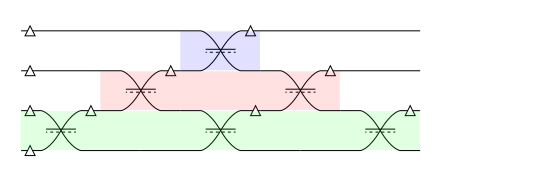
\includegraphics{figures/example}
  \caption{A \(6 \by 6\) unitary, expressed in linear optics according to the
    scheme in \cite{re-prl-73-58}, and the appropriate \pdf{}s for choosing
    parameters for a Haar unitary. The reflectivities of the bottom three
    beamsplitters (shaded cyan) can be chosen uniformly from the
    interval \(\left[ 0,1 \right)\), while those on higher rows are chosen from
    according to polynomials increasingly biased towards lower reflectivities.}
  \label{fig:example}
\end{figure*}

\section{qubits}
  
\section{conlusion}
We have shown how to express the probability density function for Haar random
unitary matrices in terms of physically motivated parameters. The expression is
compact and non-redundant, whereas the equivalent in the Cartesian basis would
be a lot more complicated. While the mathematics of this process has been known
for a long time, the link to linear-optical components has not previously been
made clear, and the proof presented here in terms of a change of basis is much
simpler than that in \cite{sp-jpa-43-385306}. Our formula will have
applications in the emerging field of Boson Sampling, where photons are
injected into large Haar unitaries to demonstrate the power of quantum systems
over classical. Using the results contained here, the unitaries can be
generated directly in terms of the linear optical components without having to
go through the process of orthogonalising a Gaussian matrix.



\bibliography{bib/dialling}

\end{document}
